%%%%%%%%%%%%%%%%%%%%%%%%%%%%%%%%%%%%%%%%%%%%%%%%%%
\documentclass[11pt]{article}\usepackage[]{graphicx}\usepackage[]{color}
%% maxwidth is the original width if it is less than linewidth
%% otherwise use linewidth (to make sure the graphics do not exceed the margin)
\makeatletter
\def\maxwidth{ %
  \ifdim\Gin@nat@width>\linewidth
    \linewidth
  \else
    \Gin@nat@width
  \fi
}
\makeatother

\definecolor{fgcolor}{rgb}{0.345, 0.345, 0.345}
\newcommand{\hlnum}[1]{\textcolor[rgb]{0.686,0.059,0.569}{#1}}%
\newcommand{\hlstr}[1]{\textcolor[rgb]{0.192,0.494,0.8}{#1}}%
\newcommand{\hlcom}[1]{\textcolor[rgb]{0.678,0.584,0.686}{\textit{#1}}}%
\newcommand{\hlopt}[1]{\textcolor[rgb]{0,0,0}{#1}}%
\newcommand{\hlstd}[1]{\textcolor[rgb]{0.345,0.345,0.345}{#1}}%
\newcommand{\hlkwa}[1]{\textcolor[rgb]{0.161,0.373,0.58}{\textbf{#1}}}%
\newcommand{\hlkwb}[1]{\textcolor[rgb]{0.69,0.353,0.396}{#1}}%
\newcommand{\hlkwc}[1]{\textcolor[rgb]{0.333,0.667,0.333}{#1}}%
\newcommand{\hlkwd}[1]{\textcolor[rgb]{0.737,0.353,0.396}{\textbf{#1}}}%

\usepackage{framed}
\makeatletter
\newenvironment{kframe}{%
 \def\at@end@of@kframe{}%
 \ifinner\ifhmode%
  \def\at@end@of@kframe{\end{minipage}}%
  \begin{minipage}{\columnwidth}%
 \fi\fi%
 \def\FrameCommand##1{\hskip\@totalleftmargin \hskip-\fboxsep
 \colorbox{shadecolor}{##1}\hskip-\fboxsep
     % There is no \\@totalrightmargin, so:
     \hskip-\linewidth \hskip-\@totalleftmargin \hskip\columnwidth}%
 \MakeFramed {\advance\hsize-\width
   \@totalleftmargin\z@ \linewidth\hsize
   \@setminipage}}%
 {\par\unskip\endMakeFramed%
 \at@end@of@kframe}
\makeatother

\definecolor{shadecolor}{rgb}{.97, .97, .97}
\definecolor{messagecolor}{rgb}{0, 0, 0}
\definecolor{warningcolor}{rgb}{1, 0, 1}
\definecolor{errorcolor}{rgb}{1, 0, 0}
\newenvironment{knitrout}{}{} % an empty environment to be redefined in TeX

\usepackage{alltt}
%%%%%%%%%%%%%%%%%%%%%%%%%%%%%%%%%%%%%%%%%%%%%%%%%%

%packages
\usepackage{amsmath,amssymb,graphicx,amsfonts,psfrag,layout,subfigure,array,longtable,lscape,booktabs,dcolumn,hyperref}
\usepackage{natbib}
\usepackage[page]{appendix}
\usepackage{multicol}  
\usepackage{setspace}
\usepackage{hyperref, url}
\usepackage[margin=1in]{geometry} %1 inch margins
\usepackage{gensymb}

%change encoding
\usepackage[utf8]{inputenc}

%code chunk margins
\usepackage{listings}

%macros
\newcommand{\Adv}{{\mathbf{Adv}}}       
\newcommand{\prp}{{\mathrm{prp}}}                  
\newcommand{\calK}{{\cal K}}
\newcommand{\outputs}{{\Rightarrow}}                
\newcommand{\getsr}{{\:\stackrel{{\scriptscriptstyle\hspace{0.2em}\$}}{\leftarrow}\:}}
\newcommand{\andthen}{{\::\;\;}}    %  \: \; for thinspace, medspace, thickspace
\newcommand{\Rand}[1]{{\mathrm{Rand}[{#1}]}}       % A command with one argument
\newcommand{\Perm}[1]{{\mathrm{Perm}[{#1}]}}       
\newcommand{\Randd}[2]{{\mathrm{Rand}[{#1},{#2}]}} % and with two arguments
\newcommand{\E}{\mathrm{E}}
\newcommand{\Var}{\mathrm{Var}}
\newcommand{\Cov}{\mathrm{Cov}}
\DeclareMathOperator*{\plim}{plim}

%%%%%%%%%%%%%%%%%%%%%%%%%%%%%%%%%%%%%%%%%%%%%%%%%%
\IfFileExists{upquote.sty}{\usepackage{upquote}}{}
\begin{document}
\title{Lab 4 - Cloud Data\\
Stat 215A, Fall 2014}
\date{\today}
\author{Tim Meyers, Jason Poulos, and Zhao Ruan \\
\\
\url{https://github.com/jvpoulos/stat215a-lab4}}
\maketitle
%%%%%%%%%%%%%%%%%%%%%%%%%%%%%%%%%%%%%%%%%%%%%%%%%%





\section{Exploratory Data Analysis}

Figure \ref{fig:map-plot-labels} spatially plots the expert labels for the presence or absence of clouds, for each of the three MISR images. In these plots, darker colors represent cloud labels, lighter colors represent no label, and white space represents non--cloud labels. 

Figure \ref{fig:plot-radiance} includes spatial plots of the radiances of each angle and Figure \ref{fig:plot-cor} is a heat map showing the correlations between radiance angles. The spatial plots of radiance angles are almost indistinguishable. Each radiance angle pair are highly correlated (over 0.5 correlation value), although some angles are more correlated than others (e.g.,$an$ is much more correlated with $af$ than it is with $df$.)

How well do the radiance angles and features (i.e., $CORR$, $NSAI$, and $SD$) predict the presence or absence of clouds? Figure \ref{fig:logistic-plots} plots the probabilities from two logistic regression models predicting an indicator variable for the presence of clouds, with radiance angles (left plot) and features (right plot) as regressors. For each regression model, we estimate the predicted probablities for each pixel, and arrange the probabilities in ascending order. We then plot the probablities for each pixel (black line) and show which pixels are labeled cloud (red lines). The plots demonstrate that both models fit the data well, given that most of the cloud labels are clustered at the right--hand side of the graphs. However, the features model provides a much better overall fit of the data since all the cloud labels are clustered a the right--hand side.



\begin{knitrout}
\definecolor{shadecolor}{rgb}{0.969, 0.969, 0.969}\color{fgcolor}\begin{figure}[]

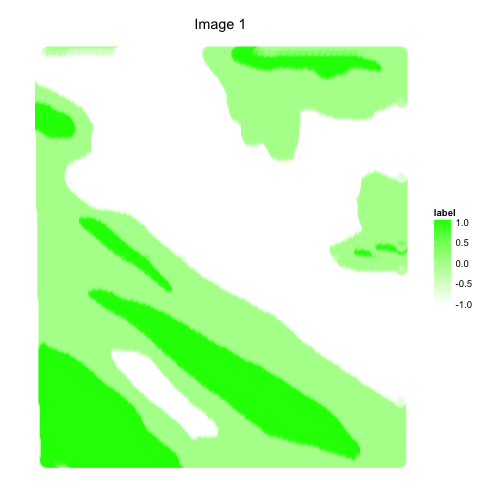
\includegraphics[width=0.49\linewidth]{figure/map-plot-labels-1} 
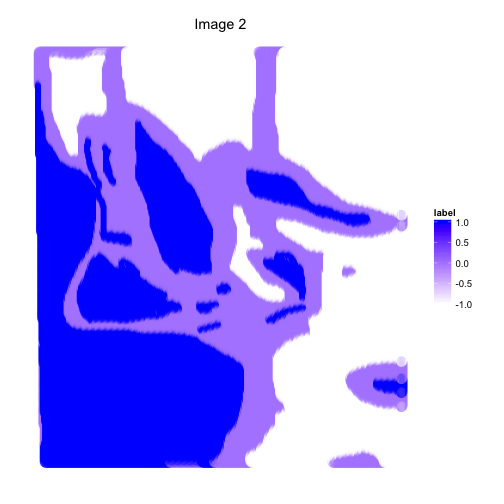
\includegraphics[width=0.49\linewidth]{figure/map-plot-labels-2} 
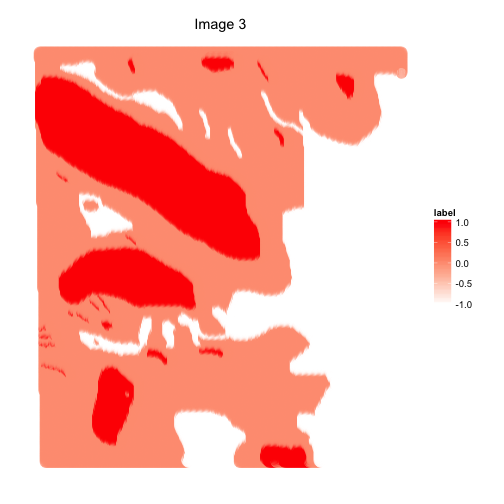
\includegraphics[width=0.49\linewidth]{figure/map-plot-labels-3} \caption[Spatial plot of the expert labels for the presence or absence of clouds, for each MISR image]{Spatial plot of the expert labels for the presence or absence of clouds, for each MISR image.\label{fig:map-plot-labels}}
\end{figure}


\end{knitrout}

\begin{knitrout}
\definecolor{shadecolor}{rgb}{0.969, 0.969, 0.969}\color{fgcolor}\begin{figure}[]

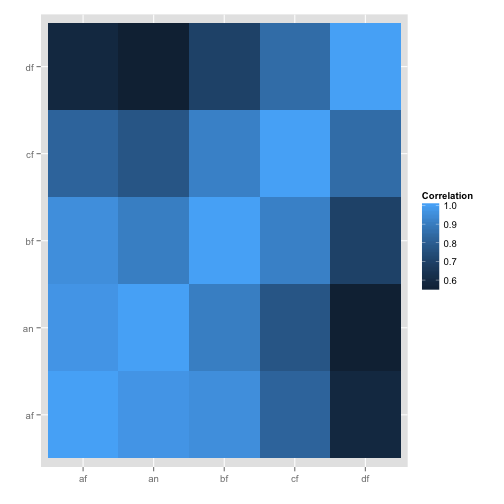
\includegraphics[width=0.49\linewidth]{figure/plot-cor-1} \caption[Radiance angle correlations]{Radiance angle correlations.\label{fig:plot-cor}}
\end{figure}


\end{knitrout}

\begin{knitrout}
\definecolor{shadecolor}{rgb}{0.969, 0.969, 0.969}\color{fgcolor}\begin{figure}[]

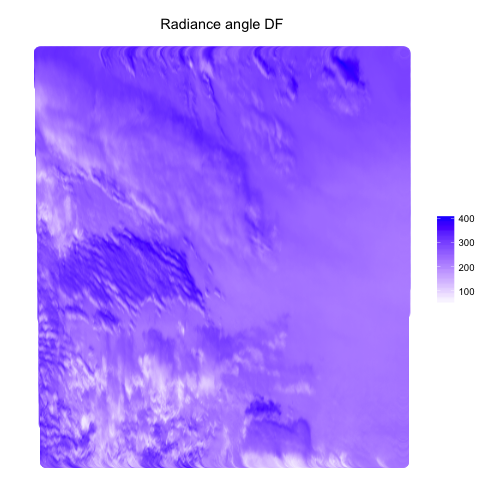
\includegraphics[width=0.49\linewidth]{figure/plot-radiance-1} 
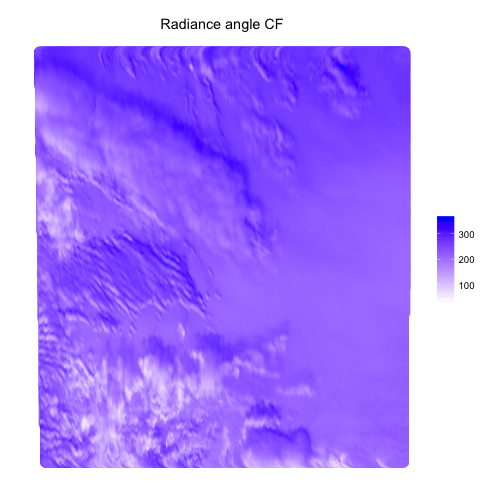
\includegraphics[width=0.49\linewidth]{figure/plot-radiance-2} 
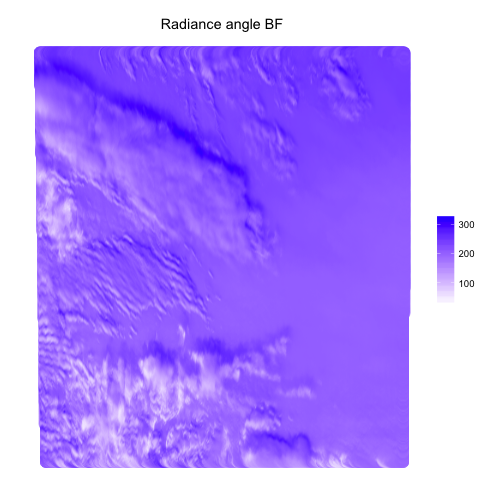
\includegraphics[width=0.49\linewidth]{figure/plot-radiance-3} 
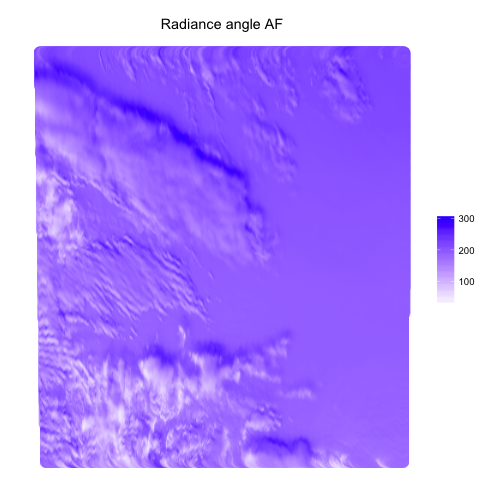
\includegraphics[width=0.49\linewidth]{figure/plot-radiance-4} 
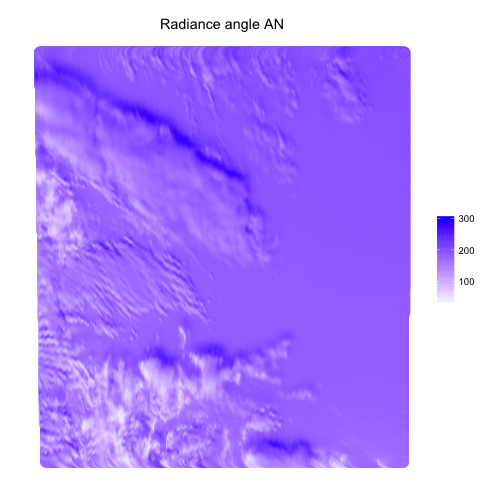
\includegraphics[width=0.49\linewidth]{figure/plot-radiance-5} \caption[Spatial plot of each radiance angle]{Spatial plot of each radiance angle.\label{fig:plot-radiance}}
\end{figure}


\end{knitrout}

\begin{knitrout}
\definecolor{shadecolor}{rgb}{0.969, 0.969, 0.969}\color{fgcolor}\begin{figure}[]

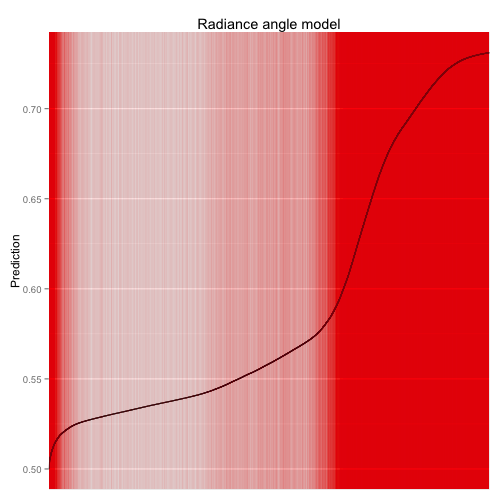
\includegraphics[width=0.49\linewidth]{figure/logistic-plots-1} 
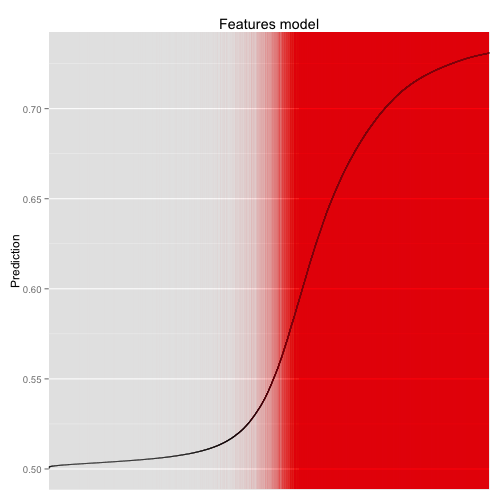
\includegraphics[width=0.49\linewidth]{figure/logistic-plots-2} \caption[Plot of probabilities from logistic regression model predicting expert label for the presence of clouds, with radiance angles (L) and features (R) as regressors]{Plot of probabilities from logistic regression model predicting expert label for the presence of clouds, with radiance angles (L) and features (R) as regressors. Predicted probablities are arranged in ascending order. Red lines correspond to actual cloud labels and the black line represents predicted probabilities for each pixel. The plots are designed to visualize the overall fit of the corresponding model.\label{fig:logistic-plots}}
\end{figure}


\end{knitrout}


\end{document}
